\section{Information View}

\begin{figure}[H]
    \centering
    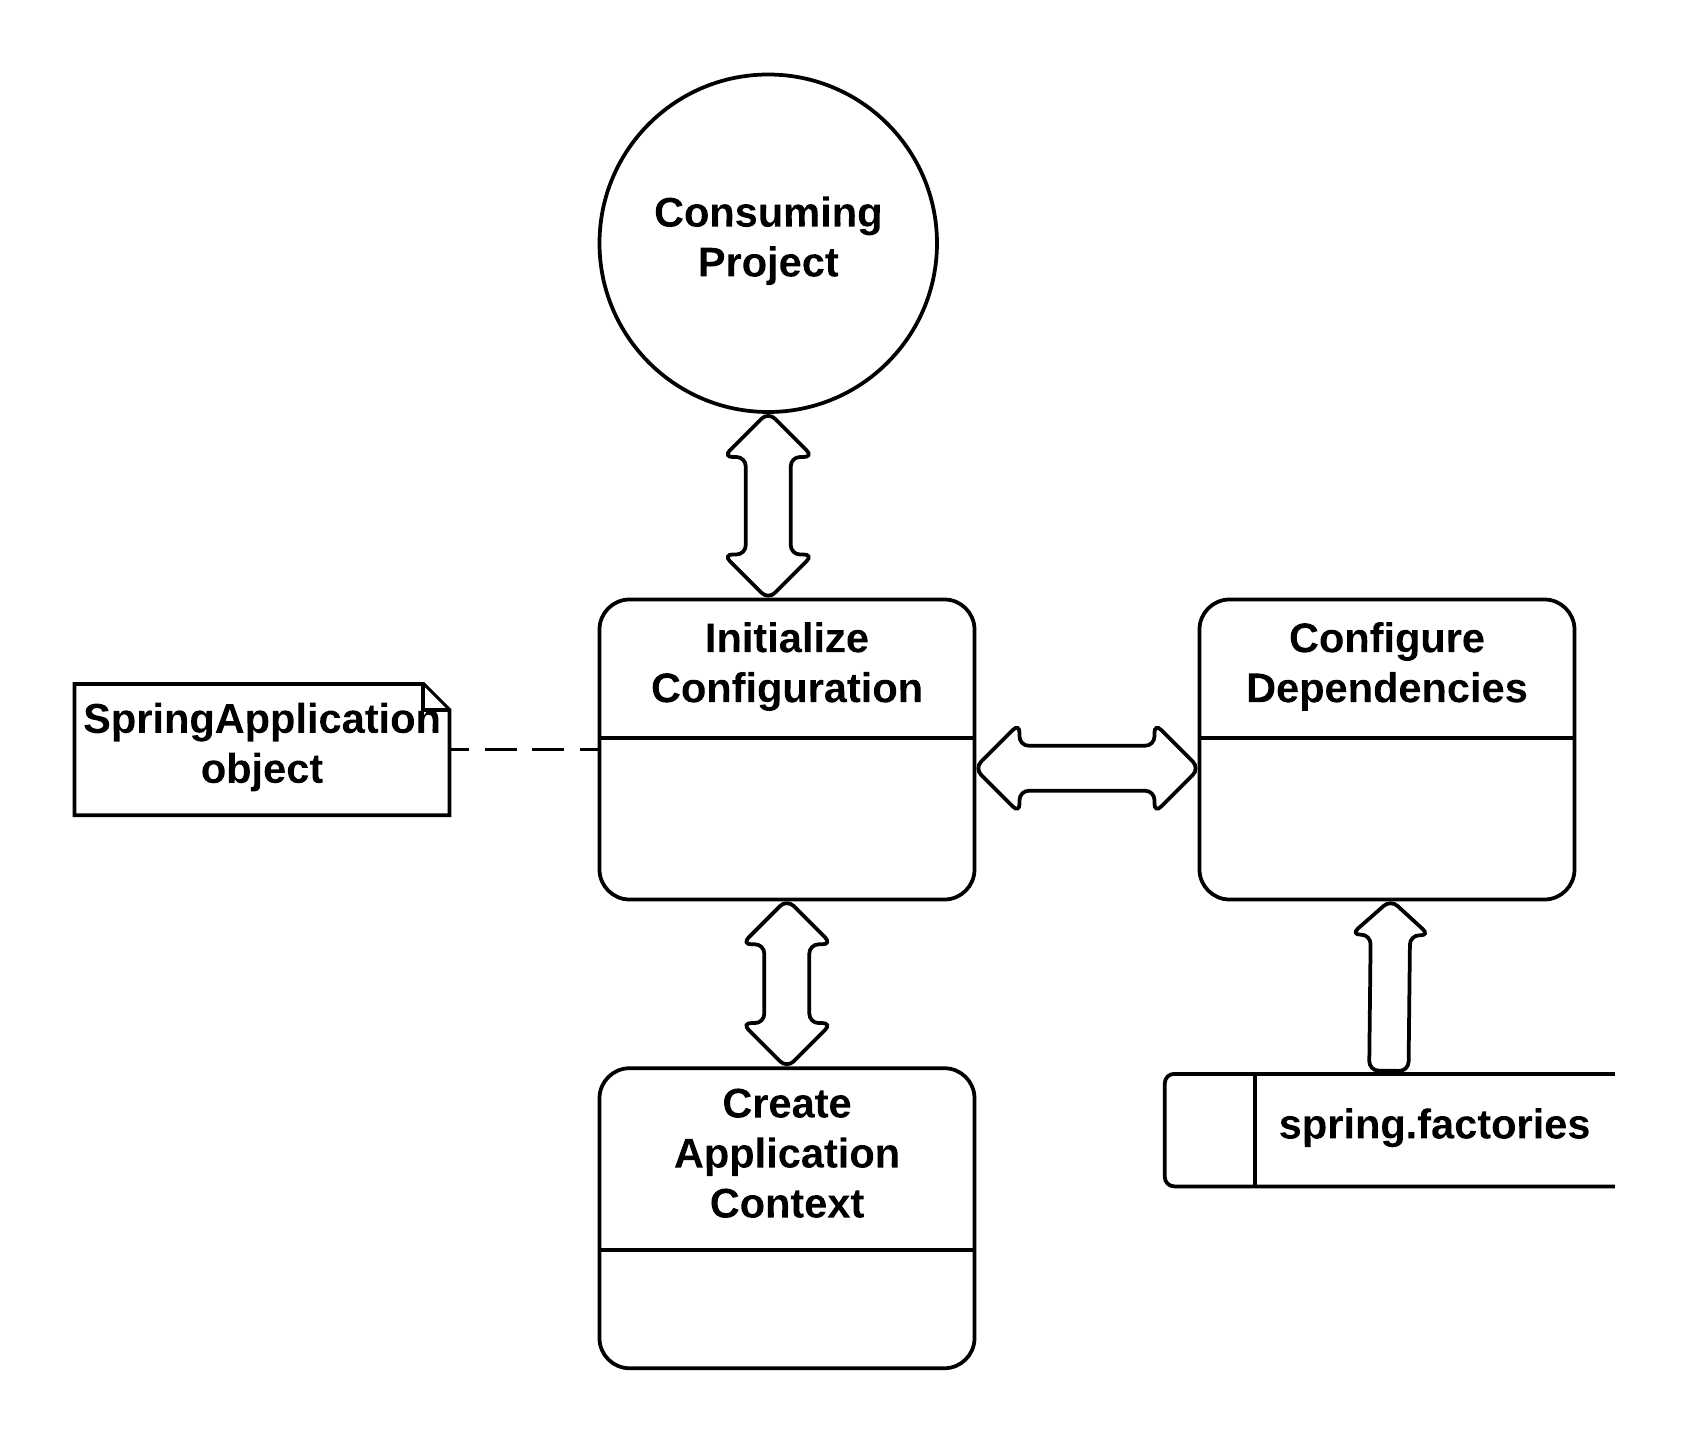
\includegraphics[width=.75\textwidth]{content/architectural-views-top-level/information-flow.png}
    \caption{Spring Boot Configuration Information Flow}
    \label{information-flow-diagram}
\end{figure}

Figure~\ref{information-flow-diagram} shows how data flows throughout a consuming project to auto-configure dependencies. The information flow can be described as the following:

\begin{enumerate}
\item The consuming project as the external entity provides dependencies from its' classpath to the \texttt{SpringApplication} object which initializes the configuration process.
\item The web application type is determined by the classpath dependencies -- of which those dependencies are loaded from the \texttt{ClassLoader} -- which then is passed around to create the application context.
\item Once the application context is created, it will be refreshed to configure dependencies based on the pre-defined list of auto-configuration classes.
\item During the auto-configuration in the configure dependencies process, the list is read from the spring.factories and matched against the loaded classpath dependencies and auto-configure them into beans.
\item Once all of the necessary beans are created, the application context will again refresh to load in all of the beans and return to the \texttt{SpringApplication} object which passes the application context to the consuming project.
\end{enumerate}

\begin{figure}[H]
    \centering
    \includegraphics[width=.7\textwidth]{content/architectural-views-top-level/information-lifecycle.png}
    \caption{Spring Boot Configuration Information Lifecycle}
    \label{information-lifecycle-diagram}
\end{figure}

Figure~\ref{information-lifecycle-diagram} shows the Spring Boot auto-configuration lifecycle, which is simple from a high level view. Once the application context is created, and then the application context is refreshed to configure dependencies. Once those dependencies are configured, the application context again is refreshed and the lifecycle ends.\\

\subsection{Data Quality}

\textbf{Timeliness and Latency}: The Spring Boot module and the data on which it manipulates is essentially static data after its' runtime processes are finished. Spring Boot will be able to use the new data as soon as the application is restarted. Consider the following scenario:

\begin{quote}
\textit{The consuming project has third-party dependencies used in a dependency management tool. When the consuming project starts up and the Spring Boot module is able to use the dependencies to help configure dependencies. While the application is up and running, the user decides to make changes in the dependency management tool, however, the changes are not reflected during this time.}
\end{quote}

The consuming project has to be restarted in this situation to reflect the changes made in dependency management tool. These changes will also be reflected in the configuration that Spring Boot behind the scene.\\

\textbf{Archiving and Information Retention}: Archiving and information retention is not important in Spring Boot module as it depends on the consuming project to provide the data for configuration. It is up to the consuming project on how they manage the data and then Spring Boot can then leverage that to help in configuration.\\

\textbf{Information Quality}: As the consuming project modifies the dependencies in the dependency management tool, the information in terms of configuration will not be reflected unless the consuming project is started up or restarted. In terms of information quality, we would say it is moderate as it updates the configuration on the next application start-up but not in real-time.
